\chapter{Anatomy}\label{ch:anatomy}

\chapterCoverImage{anatomy}

As with every practice dealing with the human body, a basic \textbf{understanding} of the anatomy is mandatory, adding a tremendous benefit for the practitioner-student and also gets handy with \textbf{communication}.
The field of anatomy is huge, and it doesn't need to be studied in-depth, of course.
Making yourself familiar with a few, important medical terms and the basic concepts of the human body, to also have a theoretical understanding of what's happening during the dance while enables you to see things in a broader context.

\section{Terminology}\label{sec:terminology}

The wording used in anatomy/medicine is built from sub-elements (which usually originated from Latin), thus:
Learning first the elements, and then putting them together to be able to infer the meaning of more complex, compound terms.

\subsection{Orientation}

Because a person can stand, sit, lie, or be in all kinds of positions, it is necessary to have an absolute frame of reference to provide orientation instructions.
When someone uses simple language like ``up'' or ``front'', it is not entirely clear what is actually meant, thus the following anatomical terms lead to a more \textbf{non-ambiguous language}.

\begin{itemize*}
    \item \textbf{anterior/posterior} = front/back
    \item \textbf{ventral/dorsal} = front/back of the torso
    \item \textbf{superior/inferior} = above/below
    \item \textbf{cranial/caudal} = head-/tail-wards
    \item \textbf{proximal/distal} = towards to/away from center
    \item \textbf{medial/lateral} = towards/away from the midline
    \item \textbf{superficial/profound} = more outside/inside the body
\end{itemize*}

\subsection{Movements}

Each body part can move in certain ways and directions based on the type of joint (see below) and how muscles pull on it.
Again, instructing someone to ``move up'' is ambiguous, whereas ``flex the right knee'' is clear as it can be.

\begin{itemize*}
    \item \textbf{extension/flexion} = making the angle of a joint bigger / smaller (or: stretch/bend)
    \item \textbf{internal/external (medial/lateral) rotation} = arm / leg rotating in the shoulder/hip-joint; counter-/clockwise towards to/away from the body
    \item \textbf{adduction/abduction} = moving towards or away from the body / midline
    \item \textbf{elevation/depression} = moving (shoulder) superior / inferior direction
    \item \textbf{pronation/supination} = rotating forearm so that palm facing up/down
    \item \textbf{dorsi-/plantar-flexion} = move the ankle towards the dorsum (superior surface, up) or plantar (sole, down) also often called ``point''
    \item \textbf{in-/eversion} = move the sole towards, inwards / away from the median plane, inwards
    \item \textbf{opposition/reposition} = thumb and little finger together / spread
    \item \textbf{pro-/retraction} = anterolateral / posteromedial movement of the scapula (move shoulder forward/backward)
    \item \textbf{circumduction} = conical (not really circular) movement of a limb extending from the joint it's moved by
\end{itemize*}

If we take for example a simple shoulder roll, it can be dissected in four movements: elevation, retraction, depression, and protraction.
Or similar with drawing circles with the toes, moving the ankle: dorsi-flexion, eversion, plantar-flexion, and inversion.

Terms derived from lateral movement include:

\begin{itemize*}
    \item \textbf{Uni-lateral} = ``\textit{unus}'' meaning ``one'', on one side of the body
    \item \textbf{Bi-lateral} = ``bis'' meaning ``twice'', on both sides of the body
    \item \textbf{Homo-(Ipsi-)lateral} = ``\textit{ipse}'' meaning ``same''
    \item \textbf{Contra-lateral} = ``contra'' meaning ``against'', e.g. arm on one side, and leg on the other side, creating a diagonal, like we do while walking; also one hemisphere of the brain is controlling the other side of the body
\end{itemize*}

Sometimes the Latin word for left (``sinister'') and right (``dexter'') are being used instead.
Check the next time you have a medical report available, like an X-ray, and you will see these terms pop up; consider yourself a nerd from now on.

\section{Structures}\label{sec:structures}

Next to being familiar with the very basic words of positions and directions, we also need to be able to refer to concrete structures (bones and muscles) which can be located in relation to each other and moved in a specific way.
Make yourself thus familiar with some (by far not all) anatomical terms, which help you further understand this medical jargon.

\subsection{Bones}\label{subsec:bones}

The human body has \textbf{206 bones} we can (usually) enumerate; yet by birth we have a few more, up to 280.
The head and trunk (the axial skeleton) make up 80 bones and the limbs (the appendicular skeleton) the other 126.
There are 27 bones for each hand (19 for phalanges plus metacarpals, and 8 carpals), and 26 for each foot (phalanges, metatarsals, and tarsals).

\begin{itemize*}
    \item \textbf{atlas and axis} = two top most cervical vertebrae (top part of the spine)
    \item \textbf{clavicle} = the collar bone
    \item \textbf{coccyx} = the tailbone (last part of the spine)
    \item \textbf{cranium} = the skull (cervical = neck)
    \item \textbf{patella} = the knee cap
    \item \textbf{processus} = a bony thing bulging out, usually for tendons to attach to
    \item \textbf{ribs} = true ribs (1-7, sternum connection), false ribs (8-10/12, cartilage), and floating ribs (11-12, no connection)
    \item \textbf{scapula} = the shoulder blade
    \item \textbf{sacrum} = big triangular bone at the base of the spine
    \item \textbf{SIAS} = Spina Illiaca Anterior Superior (front top pointy bone structure of the pelvis)
    \item \textbf{spina} = the spine, consisting of 33 vertebrae: 7 cervical, 12 thoracic, 5 lumbar, 5 fused sacral, 4 fused forming the coccyx
    \item \textbf{sternum} = the chest bone
\end{itemize*}

\subsection{Muscles}\label{subsec:muscles}

There are \textbf{between 600 and 840 muscles} within the typical human body, depending on how they are counted, and some variations due to mutations.

\begin{itemize*}
    \item \textbf{abs} = abdominal muscles with 3 layers wrapped around the belly
    \item \textbf{core muscles} = basically everything attached to the spine
    \item \textbf{diaphragm} = muscle for breathing at the bottom of the ribs
    \item \textbf{glutes} = buttocks consisting of gluteus maximus, medius, and minimus
    \item \textbf{obliques} = part of the core, at the sides of the abs
    \item \textbf{pectoralis} = the chest muscle (major and minor)
    \item \textbf{pelvic floor} = similar to diaphragm but at the bottom of the torso
    \item ``\textbf{stomach muscles}'' = the stomach is an organ, which indeed has (involuntary) muscles, but it's located on the left side underneath the ribs, and should not be confused with the abs / lower belly!
    \item \textbf{trapezius} = at top shoulder around the neck
    \item \textbf{transverse} = part of the core, like a belt around it
\end{itemize*}

\section{Planes}\label{sec:planes}

\begin{wrapfigure}{R}{0.3\textwidth}
    \centering
    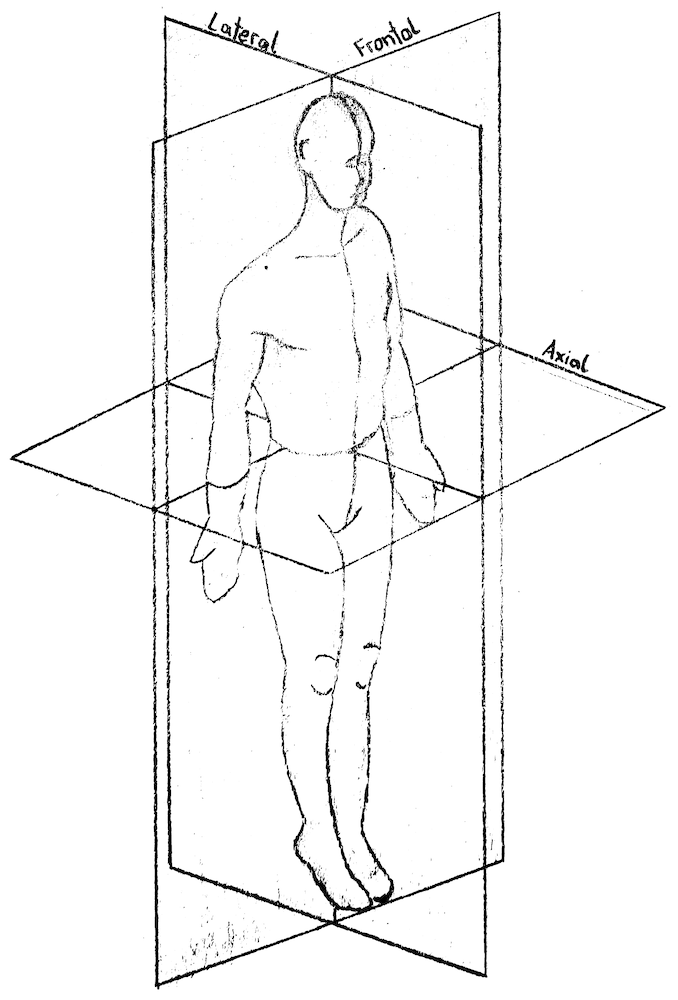
\includegraphics[width=0.3\textwidth]{images/anatomy/planes}
    \caption{The three anatomic \textbf{planes} for the human body.}
\end{wrapfigure}

We differentiate 3 different anatomical planes in which movement can happen:

\begin{enumerate}
    \item \textbf{Frontal Plane}: Also called \textit{Coronal Plane} or \textit{Vertical Plane} and, not surprisingly, represents the plane when looking from the front of the body, dividing the body into an anterior/posterior part.
    The directions can be medial/lateral, thus resulting in the movements of ad-/abduction, elevation/depression and in-/eversion.
    \item \textbf{Lateral Plane}: Also called \textit{Sagittal Plane}, \textit{Longitudinal Plane} or \textit{Anteroposterior Plane}, which is going through the midline and shows the body when looking from the side, separating it into a left/right part.
    The directions are thus anterior/posterior and movements are flexion/extension and pro-/retraction.
    \item \textbf{Axial Plane}: Also called \textit{Transverse Plane}, \textit{Horizontal Plane} (the other two planes are vertical) or \textit{Cross-Sectional Plane}, and divides the body into a top/bottom part.
    Directions are thus superior/inferior and allowing movements like rotation, supination/pronation and circumduction.
\end{enumerate}

\section{Joints}\label{sec:joints}

Bones are connected through joints where muscles (together with tendons) can evoke movement.
For different movements, \textbf{different types} of (synovial) joints are needed:

\begin{itemize*}
    \item \textbf{Ball/Socket}: free movement; e.g. hip, shoulder
    \item \textbf{Pivot}: rotation; head (atlantoaxial), elbow (radioulnar)
    \item \textbf{Hinge}: flexion/extension; elbow (humeroulnar), knee
    \item \textbf{Saddle}: fingers-hand (trapeziometacarpal)
    \item \textbf{Condyloid}: fingers/wrist (metacarpophalangeal)
    \item \textbf{Plane}: hand (intercarpal) and feet (tarsal)
    \item \textbf{Gliding}: mini bones in feet
\end{itemize*}
